\section{Взаимодействие Apache Spark с JVM и интерпретатором Python.}

\begin{figure}[H]
	\centering
	\begin{minipage}[b]{0.6\textwidth}
		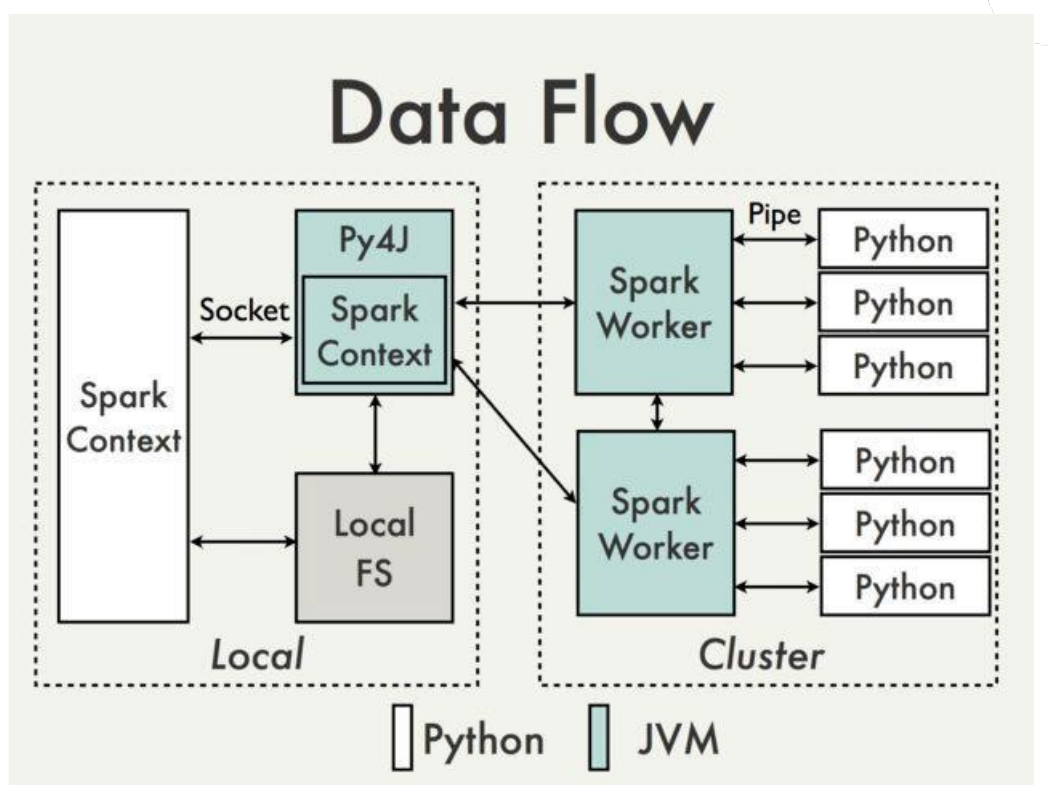
\includegraphics[width=\textwidth]{images/pyjspark.png}
		\caption{Spark python + java}
	\end{minipage}
\end{figure}

Создается питоновский spark контекст, который через сокет
стучится в джавовый спарк контекст, выставляя задачи.

Джавовый контекст достает данные из FS и пихает в java
spark worker на кластере, который выполняет питоновские
операции и отдает результаты в обратном порядке.